% ============================================================
% Apresentação (versão resumida): Sheng & Zhao (2022)
% Separação e imagem de difrações com CNN dilatada (DCNN)
% PPGEEC2327 — IA aplicada à geofísica — UFRN
% Compilar no Overleaf com pdfLaTeX
% Duração alvo: ~12–15 min (9 slides de conteúdo)
% ============================================================
\documentclass[aspectratio=169,10pt]{beamer}

\usetheme[progressbar=frametitle,numbering=fraction,block=fill,sectionpage=none]{metropolis}

\usepackage{babel}
\babelprovide[import,main]{portuguese}
\usepackage[utf8]{inputenc}
\usepackage[T1]{fontenc}
\usepackage{amsmath,amssymb,bm}
\usepackage{graphicx}
\usepackage{booktabs}
\usepackage{tikz}
\usetikzlibrary{arrows.meta,positioning}

\graphicspath{{figs/}}

% ---------- Cores (próximas aos slides da disciplina) ----------
\definecolor{verde}{HTML}{1E6B2E}
\definecolor{verdeclaro}{HTML}{E8F3EA}
\definecolor{laranja}{HTML}{C0561B}
\definecolor{laranjaclaro}{HTML}{FBEDE4}
\setbeamercolor{block title}{bg=verde,fg=white}
\setbeamercolor{block body}{bg=verdeclaro,fg=black}
\setbeamercolor{block title alerted}{bg=laranja,fg=white}
\setbeamercolor{block body alerted}{bg=laranjaclaro,fg=black}
\setbeamercolor{alerted text}{fg=laranja}

\newcommand{\fonte}[1]{\par\vspace{2pt}{\scriptsize\color{gray} Fonte: #1}}

% ---------- Estilo do fluxograma ----------
\tikzset{
  bloco/.style={draw=black, line width=1pt, rounded corners=3pt,
                minimum width=2.25cm, minimum height=1.0cm,
                align=center, font=\small\bfseries, fill=white},
  destaque/.style={bloco, fill=verdeclaro, draw=verde},
  seta/.style={-{Stealth[length=7pt]}, line width=2pt, draw=gray!70!black}
}

% \title{Separação e imagem de difrações com uma rede neural convolucional dilatada}
\title{Separation and imaging of diffractions using a dilated convolutional neural
network}
\subtitle{Sheng \& Zhao (2022), \textit{Geophysics}, 87(3), S117--S127}
\author{Matheus Augusto Monteiro da Silva \\ Raphael Ramos da Silva}
\institute{PPGEEC2327 -- IA aplicada à geofísica -- Prof. Tiago Barros -- UFRN}
\date{}

\begin{document}

\maketitle

% ============================================================
\section{Introdução}

\begin{frame}{Motivação}
  \begin{columns}[T]
    \begin{column}{0.42\textwidth}
      \begin{itemize}
        \item Difrações revelam estruturas \textbf{pequenas}: falhas, fraturas, cavidades.
        \item Reflexões, muito mais fortes, as \textbf{mascaram}.
        \item Métodos clássicos (ex.: PWD) exigem ajuste manual e falham com reflexões de \textbf{alto mergulho}.
      \end{itemize}
      \vspace{4pt}
      \begin{block}{Problema}
        \centering
        $\mathbf{y} = \mathbf{d} + \mathbf{r}$ \quad {\small (dado = difração + reflexão)}\\[2pt]
        {\small Recuperar $\mathbf{d}$ a partir de $\mathbf{y}$.}
      \end{block}
    \end{column}
    \begin{column}{0.56\textwidth}
      \centering
      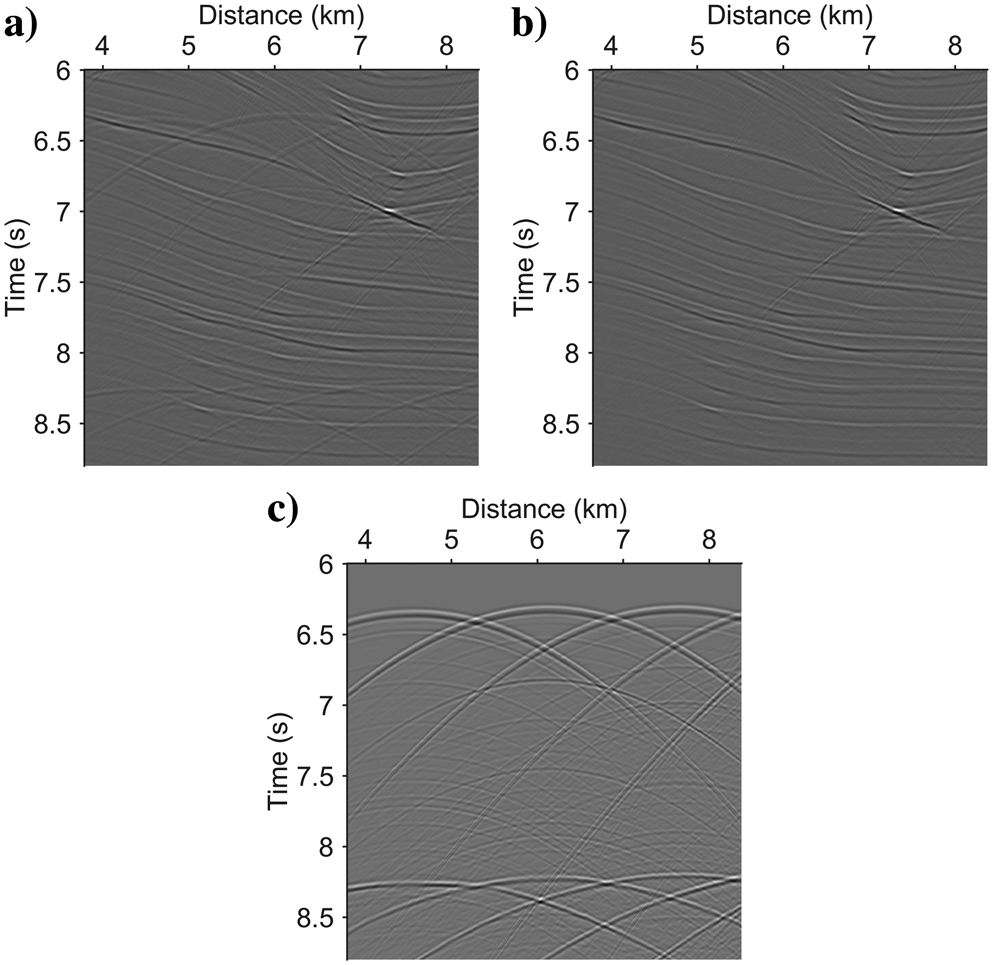
\includegraphics[width=\linewidth,height=0.71\textheight,keepaspectratio]{fig05.png}\\
      {\scriptsize (a) dado \quad (b) só reflexão \quad (c) só difração}
      \fonte{Sheng \& Zhao (2022), Fig. 5}
    \end{column}
  \end{columns}
\end{frame}

% ============================================================
\section{Metodologia}

\begin{frame}{Visão geral}
  \centering
  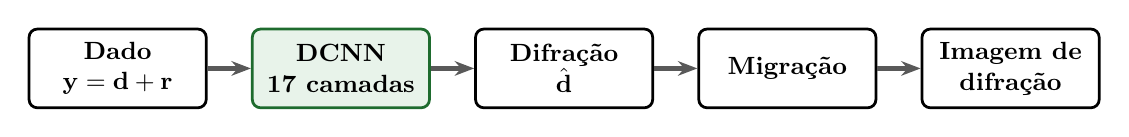
\begin{tikzpicture}[node distance=0.55cm]
    \node[bloco] (y) {Dado\\ $\mathbf{y}=\mathbf{d}+\mathbf{r}$};
    \node[destaque, right=of y] (net) {DCNN\\ 17 camadas};
    \node[bloco, right=of net] (d) {Difração\\ $\hat{\mathbf{d}}$};
    \node[bloco, right=of d] (mig) {Migração};
    \node[bloco, right=of mig] (img) {Imagem de\\ difração};
    \draw[seta] (y) -- (net);
    \draw[seta] (net) -- (d);
    \draw[seta] (d) -- (mig);
    \draw[seta] (mig) -- (img);
  \end{tikzpicture}

  \vspace{14pt}
  \begin{columns}[T]
    \begin{column}{0.48\textwidth}
      \textbf{Aprendizado supervisionado:}
      \[
        \arg\min_{\bm{\theta}} \big\| R(\mathbf{y};\bm{\theta}) - \mathbf{d} \big\|_F^2
      \]
      {\small $R$: saída da rede \quad $\bm{\theta}=\{\mathbf{W},\mathbf{b}\}$: pesos}
    \end{column}
    \begin{column}{0.48\textwidth}
      \begin{block}{Metodologia}
        \textbf{Aprendizado residual}: alvo é a parte pequena, $\mathbf{d}$\\
        \textbf{Convolução dilatada}: janela maior\\
        \textbf{Batch normalization}: treino mais rápido
      \end{block}
    \end{column}
  \end{columns}
\end{frame}

% ------------------------------------------------------------
\begin{frame}{Arquitetura e campo receptivo}
  \centering
  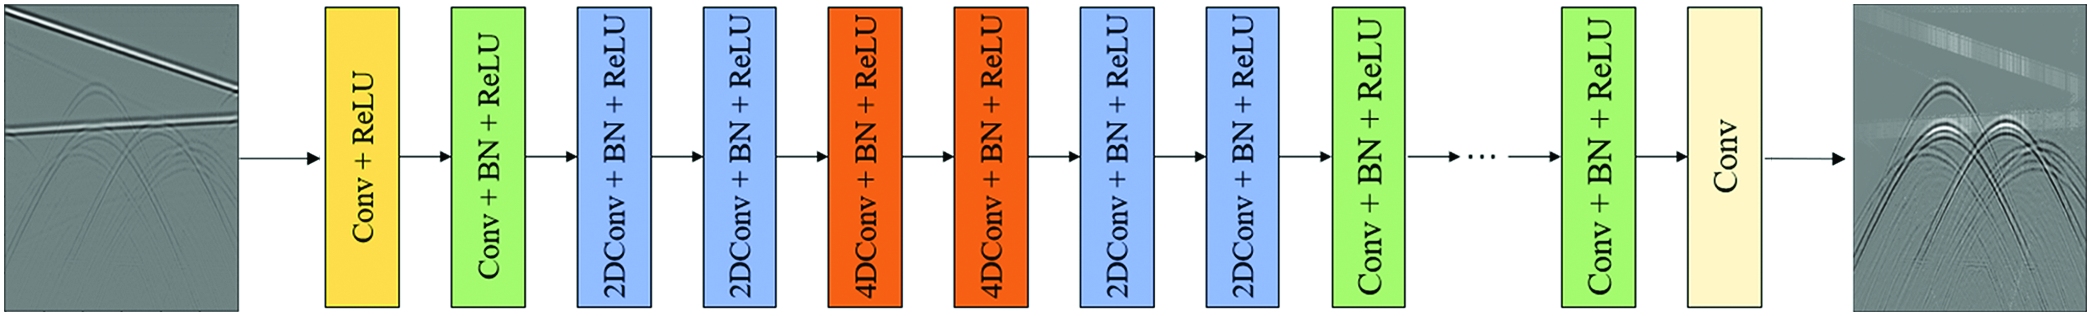
\includegraphics[width=0.82\textwidth]{fig01.png}
  \fonte{Sheng \& Zhao (2022), Fig. 1}

  \vspace{6pt}
  \begin{columns}[T]
    \begin{column}{0.3\textwidth}
      \centering
      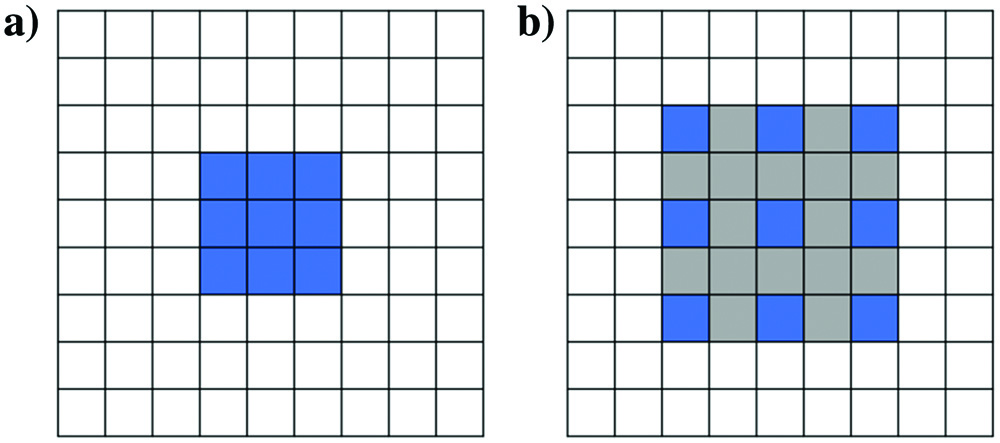
\includegraphics[width=\textwidth]{fig02.png}\\
      {\scriptsize convencional \quad dilatada}
      \fonte{Sheng \& Zhao (2022), Fig. 2}
    \end{column}
    \begin{column}{0.66\textwidth}
      \begin{itemize}
        \item Conv $3\times3$, 64 filtros, BN + ReLU; camadas 3--8 \textbf{dilatadas}.
        \item Campo receptivo: \textbf{35} (CNN comum) $\rightarrow$ \textbf{55} (DCNN), sem pesos extras.
      \end{itemize}
      \begin{block}{Ideia-chave}
        De perto, uma hipérbole parece reta; uma janela maior enxerga a \textbf{curvatura}.
      \end{block}
    \end{column}
  \end{columns}
\end{frame}

% ------------------------------------------------------------
\begin{frame}{Treinamento}
  \begin{itemize}
    \item \textbf{Função de perda}: média das perdas no lote
      \[
        l(\bm{\theta}) = \frac{1}{2N}\sum_{i=1}^{N}
        \big\| R(\mathbf{y}_i;\bm{\theta}) - \underbrace{(\mathbf{y}_i-\mathbf{r}_i)}_{\mathbf{d}_i} \big\|_F^2
      \]
    \item Otimizador \textbf{Adam} + cosine annealing com \textit{warm restart}.
    \item Dados sintéticos: gabarito por subtração (modelo com $-$ sem espalhadores).
    \item Recortes $55\times55$; lote 32; 60 épocas.
    \item Teste no \textbf{Sigsbee2A}, fora do treino.
  \end{itemize}
\end{frame}

% ------------------------------------------------------------
\begin{frame}{Treinamento: cosine annealing}
  \begin{columns}[T]
    \begin{column}{0.52\textwidth}
      \textbf{Taxa de aprendizado} na época $t$:
      \[
        \alpha_t = \alpha^j_{\min} + \tfrac{1}{2}\big(\alpha^j_{\max} - \alpha^j_{\min}\big)
        \Big(1 + \cos\Big(\tfrac{T_{\mathrm{cur}}}{T_j}\,\pi\Big)\Big)
      \]
      {\small $j$: $j$-ésimo reinício\\
      $\alpha^j_{\max}$, $\alpha^j_{\min}$: taxas máxima e mínima\\
      $T_{\mathrm{cur}}$: épocas decorridas; $T_j$: época do reinício}
      \vspace{6pt}
      \begin{alertblock}{\textit{Conventional} $\times$ \textit{Annealing}}
        \small
        \textit{Conventional}: taxa de aprendizado cai em "degraus"\\
        \textit{Annealing}: a taxa cai suavemente, em forma de cosseno, voltando a subir periodicamente (\textit{warm restart}). Esse reinício ajuda a escapar de mínimos locais e "automatiza" a atualização de $\alpha$.
      \end{alertblock}
    \end{column}
    \begin{column}{0.44\textwidth}
      \centering
      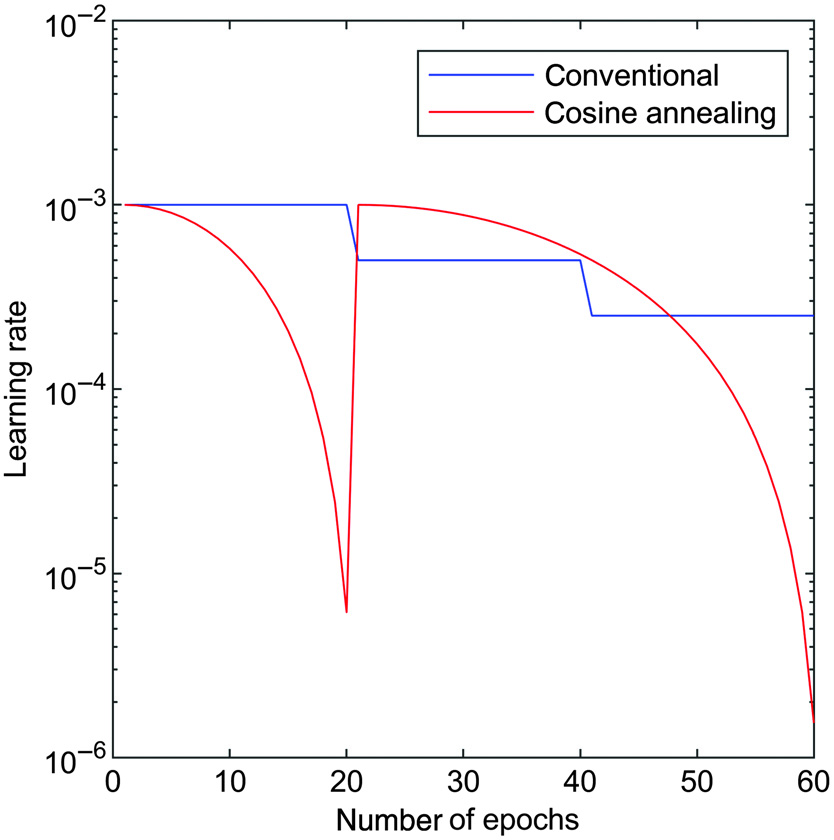
\includegraphics[height=0.6\textheight]{fig03.png}\\
      {\scriptsize taxa de aprendizado: degraus $\times$ cosseno}
      \fonte{Sheng \& Zhao (2022), Fig. 3}
    \end{column}
  \end{columns}
\end{frame}

% ============================================================
\section{Resultados sintéticos}

\begin{frame}{Sigsbee2A: PWD $\times$ DCNN}
  \begin{columns}[T]
    \begin{column}{0.52\textwidth}
      \centering
      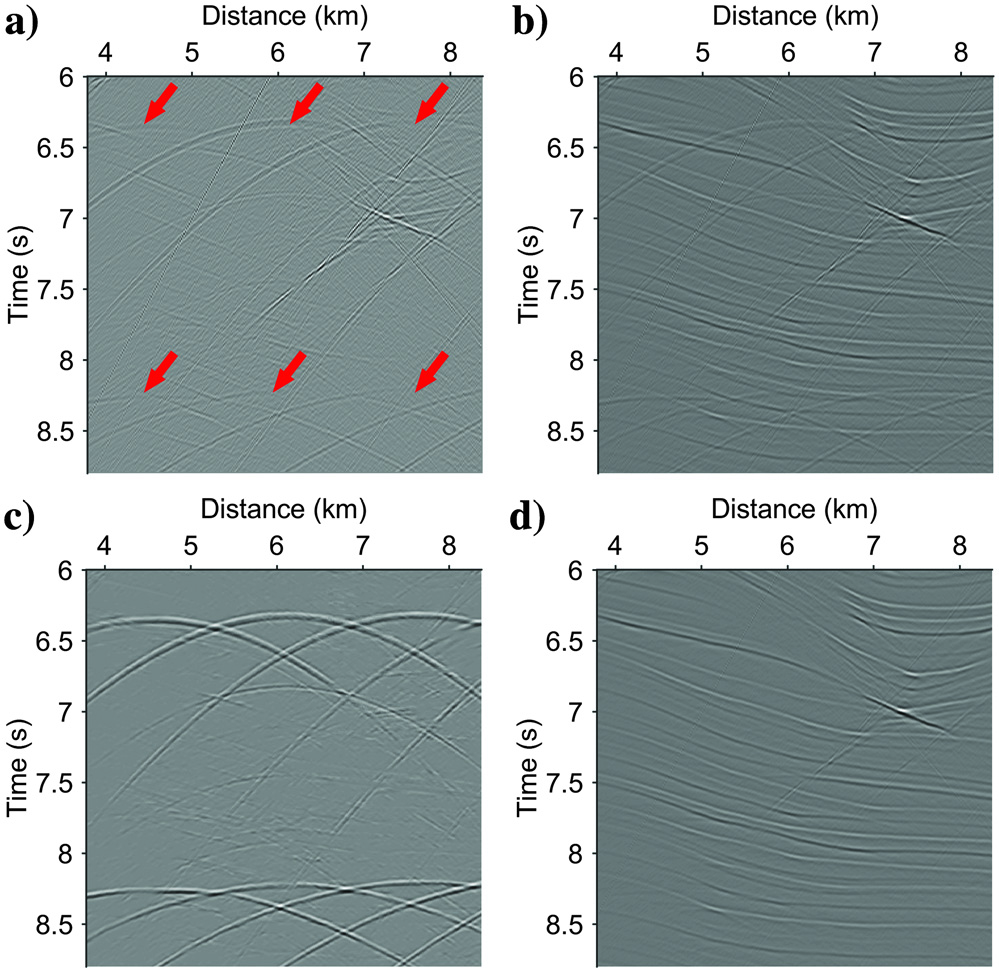
\includegraphics[width=\linewidth,height=0.71\textheight,keepaspectratio]{fig09.png}\\
      {\scriptsize (a) PWD \quad (b) resíduo \quad (c) DCNN \quad (d) resíduo}
      \fonte{Sheng \& Zhao (2022), Fig. 9}
    \end{column}
    \begin{column}{0.44\textwidth}
      \begin{itemize}
        \item PWD apaga os \alert{ápices} e trechos tangentes (setas).
        \item DCNN preserva as hipérboles inteiras.
      \end{itemize}
      \centering
      \begin{tabular}{lc}
        \toprule
        Método & EQM \\
        \midrule
        PWD  & $4{,}02\times10^{-4}$ \\
        CNN comum & $1{,}05\times10^{-4}$ \\
        DCNN & $\mathbf{3{,}59\times10^{-5}}$ \\
        \bottomrule
      \end{tabular}
      \vspace{2pt}
      \begin{block}{EQM: erro quadrático médio}
        \small
        $\text{EQM} = \frac{1}{M}\sum_{k=1}^{M}\big(\hat{d}_k - d_k\big)^2$\\[2pt]
        Erro entre difração separada $\hat{\mathbf{d}}$ e verdadeira $\mathbf{d}$.
        Menor EQM = menos \textbf{energia perdida}.
      \end{block}
    \end{column}
  \end{columns}
\end{frame}

% ------------------------------------------------------------
\begin{frame}{Sigsbee2A: imagem de difração}
  \begin{columns}[T]
    \begin{column}{0.5\textwidth}
      \centering
      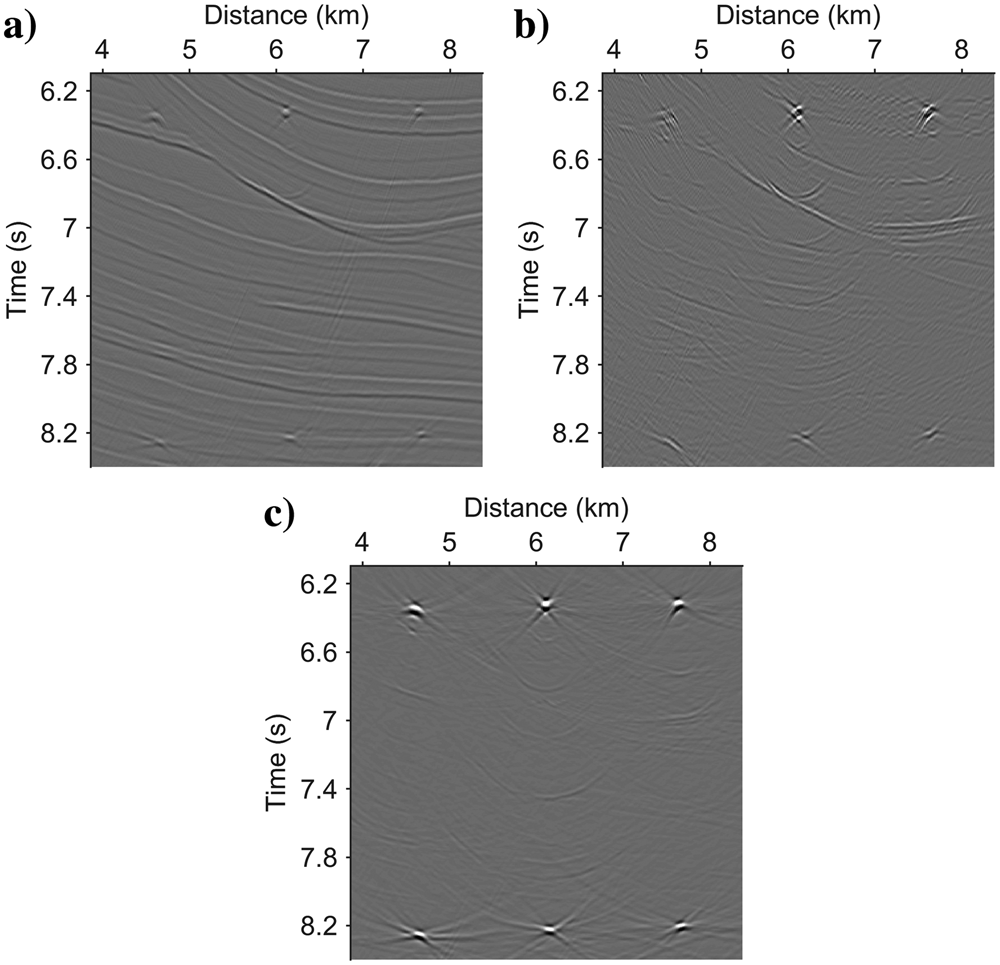
\includegraphics[width=\linewidth,height=0.775\textheight,keepaspectratio]{fig10.png}\\
      {\scriptsize\color{gray} Fonte: Sheng \& Zhao (2022), Fig. 10}
    \end{column}
    \begin{column}{0.46\textwidth}
      \begin{enumerate}[(a)]
        \item Migração convencional: espalhadores quase invisíveis.
        \item PWD: espalhadores borrados.
        \item DCNN: espalhadores \textbf{focalizados}.
      \end{enumerate}
    \end{column}
  \end{columns}
\end{frame}

% ============================================================
\section{Dado real}

\begin{frame}{Nankai: separação}
  \begin{columns}[T]
    \begin{column}{0.5\textwidth}
      \centering
      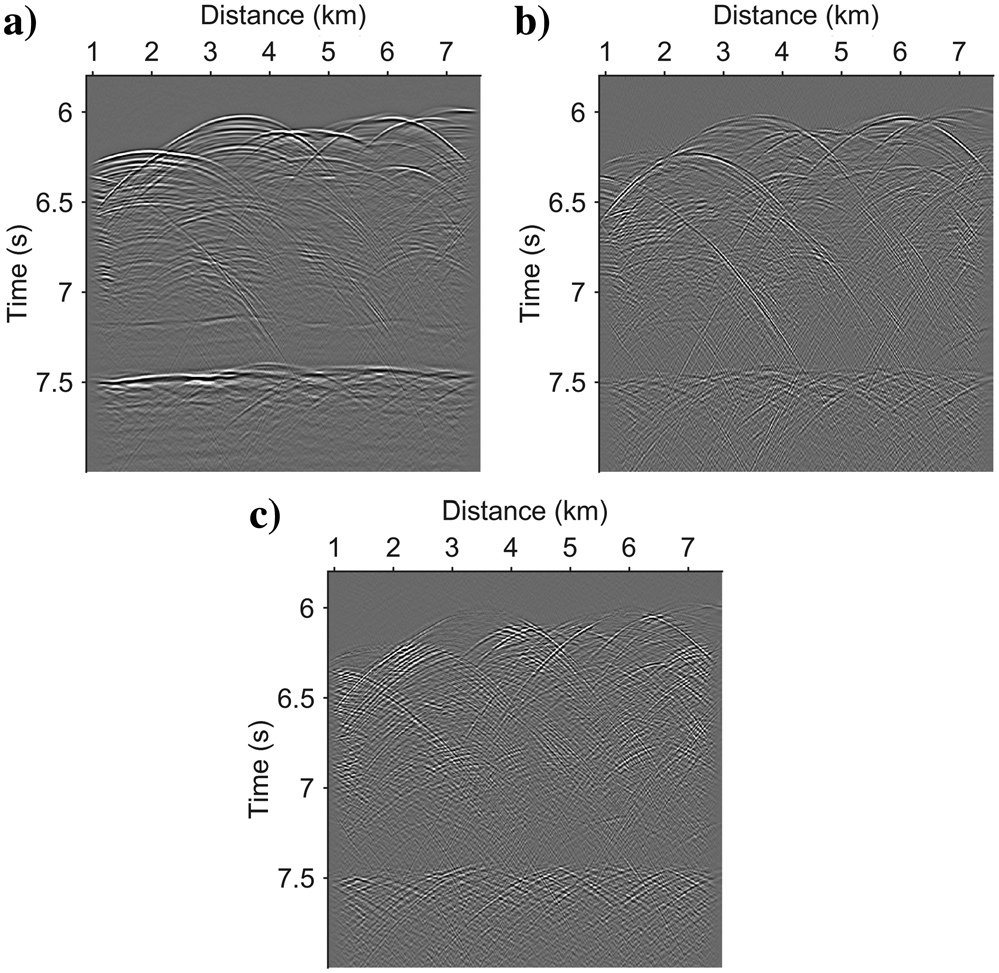
\includegraphics[width=\linewidth,height=0.71\textheight,keepaspectratio]{fig16.png}\\
      {\scriptsize (a) dado \quad (b) PWD \quad (c) DCNN}
      \fonte{Sheng \& Zhao (2022), Fig. 16}
    \end{column}
    \begin{column}{0.46\textwidth}
      \begin{itemize}
        \item Treino no \textbf{Viking Graben}, com rótulos gerados pelo PWD.
        \item Teste em Nankai: reflexões muito inclinadas.
        \item PWD deixa vazar reflexões; DCNN as remove melhor.
      \end{itemize}
    \end{column}
  \end{columns}
\end{frame}

% ------------------------------------------------------------
\begin{frame}{Nankai: imagem e limites}
  \begin{columns}[T]
    \begin{column}{0.5\textwidth}
      \centering
      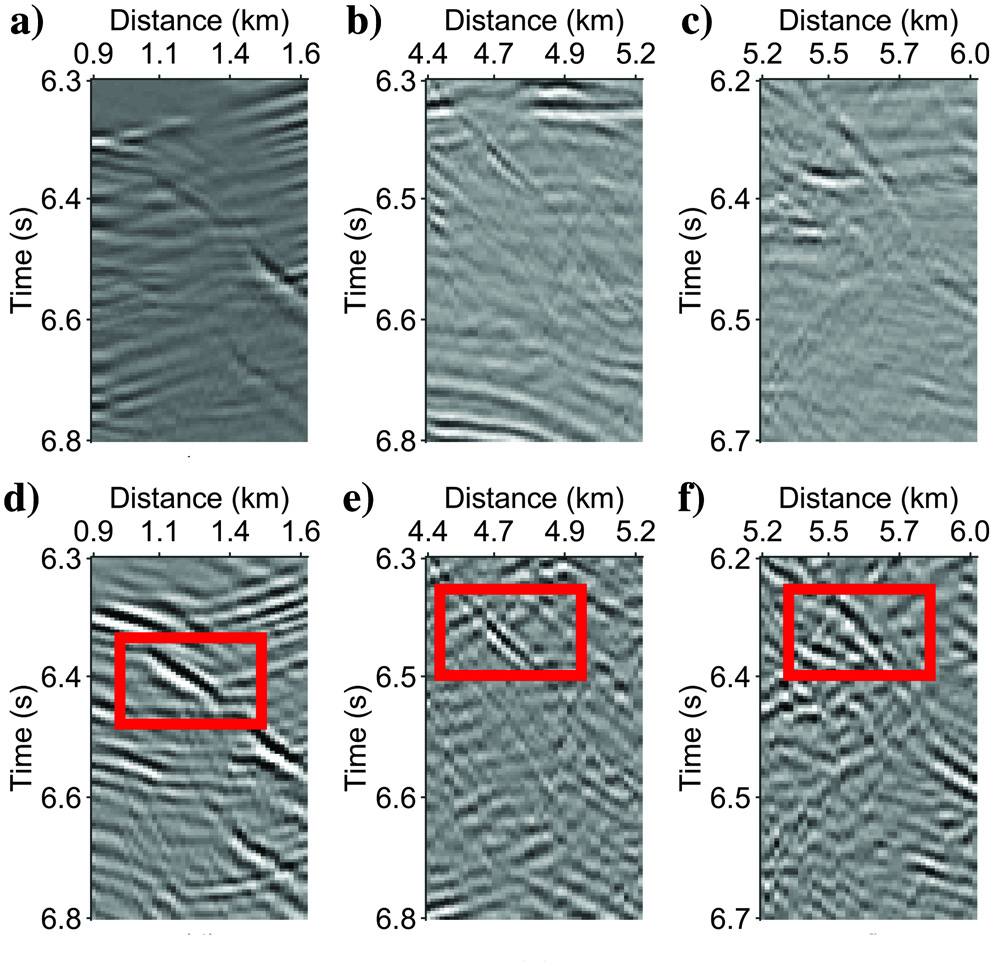
\includegraphics[height=0.58\textheight]{fig18.png}\\
      {\scriptsize (a--c) migração convencional \quad (d--f) imagem de difração}
      \fonte{Sheng \& Zhao (2022), Fig. 18}
    \end{column}
    \begin{column}{0.46\textwidth}
      \begin{itemize}
        \item Fraturas pequenas ficam visíveis (retângulos).
      \end{itemize}
      \vspace{6pt}
      \begin{alertblock}{Limite}
        Treinada só no sintético, a rede falha no campo: o treino precisa se parecer com o teste.
      \end{alertblock}
    \end{column}
  \end{columns}
\end{frame}

% ============================================================
% \section{Conclusões}
% 
% \begin{frame}{Conclusões}
%   \begin{columns}[T]
%     \begin{column}{0.5\textwidth}
%       \textbf{Contribuições}
%       \begin{itemize}
%         \item Separação sem ajuste manual após o treino.
%         \item EQM $\approx$ 11$\times$ menor que o PWD no sintético.
%         \item Realça fraturas no dado real.
%       \end{itemize}
%     \end{column}
%     \begin{column}{0.46\textwidth}
%       \textbf{Limitações}
%       \begin{itemize}
%         \item Campo avaliado só visualmente.
%         \item Rótulos de campo vêm do PWD.
%         \item Sensível à diferença treino--teste.
%       \end{itemize}
%     \end{column}
%   \end{columns}
% \end{frame}

% ------------------------------------------------------------
\begin{frame}[standout]
  Obrigado!
\end{frame}

\end{document}
